\section{Neuronale Netze}
\setcounter{aufgabe}{0}
% ===================================================================
% Aufgaben zu Neuronalen Netzen
% Themen: Perzeptron, Hebbsche Lernregel, Boolesche Funktionen,
%         Aktivierungsfunktionen, MLP-Vorwaertsrechnung,
%         Gradientenabstieg, Backpropagation
% ===================================================================

% -------------------------------------------------------------------
% 1) Perzeptron: Klassifikation und Trenngerade
% -------------------------------------------------------------------
\aufgabe{
Gegeben sei ein einlagiges Perzeptron mit einem Ausgabeneuron und dem
Eingaberaum $\mathbb{R}^2$. Der Gewichtsvektor sei
$\mathbf{w} = \begin{pmatrix} 2 \\ -1 \end{pmatrix} \in \mathbb{R}^2$, der
Schwellenwert $\theta = 1$. Die Netzeingabe ist
\[
  h : \mathbb{R}^2 \to \mathbb{R}, \qquad
  h(\mathbf{x}) = \mathbf{w} \cdot \mathbf{x},
\]
die Ausgabe $y = g\bigl(h(\mathbf{x})\bigr)$ mit der Heaviside-Funktion
\[
  g : \mathbb{R} \to \{0,1\}, \qquad
  g(h) =
  \begin{cases}
    1, & h > \theta,\\
    0, & h \leq \theta.
  \end{cases}
\]

\begin{enumerate}[label=\alph*)]
  \item Bestimmen Sie die Ausgabe für
        $\mathbf{x}_1 = \begin{pmatrix} 1 \\ 0 \end{pmatrix}$,
        $\mathbf{x}_2 = \begin{pmatrix} 0 \\ 2 \end{pmatrix}$ und
        $\mathbf{x}_3 = \begin{pmatrix} 2 \\ 3 \end{pmatrix}$.
  \item Geben Sie die Trenngerade $h(\mathbf{x}) - \theta = 0$ in der Form
        $x_2 = a\,x_1 + b$ an.
  \item Berechnen Sie den Abstand des Punktes $\mathbf{x}_1$ zur Trenngeraden.
\end{enumerate}
}

\loesung{
\begin{enumerate}[label=\alph*)]
  \item Es gilt $h(\mathbf{x}) = 2x_1 - x_2$:
  \[
    h(\mathbf{x}_1) = 2 - 0 = 2 > 1 \;\Rightarrow\; y = \textbf{1}
  \]
  \[
    h(\mathbf{x}_2) = 0 - 2 = -2 \leq 1 \;\Rightarrow\; y = \textbf{0}
  \]
  \[
    h(\mathbf{x}_3) = 4 - 3 = 1 \leq 1 \;\Rightarrow\; y = \textbf{0}
  \]
  Der Punkt $\mathbf{x}_3$ liegt genau \textbf{auf} der Trenngeraden und wird
  wegen $h \leq \theta$ der Klasse $0$ zugeordnet.

  \item Aus $2x_1 - x_2 - 1 = 0$ folgt
  \[
    x_2 = 2x_1 - 1.
  \]

  \item Mit $\lVert\mathbf{w}\rVert = \sqrt{2^2 + (-1)^2} = \sqrt{5}$:
  \[
    r = \frac{h(\mathbf{x}_1) - \theta}{\lVert\mathbf{w}\rVert}
      = \frac{2 - 1}{\sqrt{5}} \approx 0{,}447.
  \]
\end{enumerate}
}

% -------------------------------------------------------------------
% 2) Hebbsche Lernregel
% -------------------------------------------------------------------
\aufgabe{
Ein Perzeptron mit Bias-Neuron verwendet den erweiterten Eingabevektor
$\mathbf{x} = (x_0, x_1, x_2)^{\mathsf{T}}$ mit $x_0 = 1$ und den
Gewichtsvektor
\[
  \mathbf{w} = (-0{,}2;\; 0{,}5;\; -0{,}3)^{\mathsf{T}},
  \qquad \eta = 0{,}2 .
\]
Die Ausgabe ist $\hat{y} = \text{heaviside}(\mathbf{w}\cdot\mathbf{x})$, d. h.
$\hat{y} = 1$ für $\mathbf{w}\cdot\mathbf{x} > 0$, sonst $\hat{y} = 0$.

Führen Sie zwei Schritte der Hebbschen Lernregel
$\Delta w_j = \eta\cdot\text{error}\cdot x_j$ durch:

\begin{enumerate}[label=\alph*)]
  \item Beispiel $\mathbf{x} = (1, 1, 1)^{\mathsf{T}}$ mit $y = 1$.
  \item Beispiel $\mathbf{x} = (1, 1, 0)^{\mathsf{T}}$ mit $y = 0$.
  \item Geben Sie die resultierende Trenngerade in der Form
        $x_2 = a\,x_1 + b$ an.
\end{enumerate}
}

\loesung{
\begin{enumerate}[label=\alph*)]
  \item Netzeingabe:
  \[
    \mathbf{w}\cdot\mathbf{x} = -0{,}2 + 0{,}5 - 0{,}3 = 0
    \;\Rightarrow\; \hat{y} = 0, \qquad \text{error} = 1 - 0 = 1 .
  \]
  Gewichtsänderungen:
  \[
    \Delta w_j = 0{,}2\cdot 1\cdot x_j = 0{,}2
    \quad\text{für } j = 0,1,2
  \]
  \[
    \mathbf{w} = (0;\; 0{,}7;\; -0{,}1)^{\mathsf{T}}
  \]

  \item Netzeingabe:
  \[
    \mathbf{w}\cdot\mathbf{x} = 0 + 0{,}7 + 0 = 0{,}7 > 0
    \;\Rightarrow\; \hat{y} = 1, \qquad \text{error} = 0 - 1 = -1 .
  \]
  Gewichtsänderungen:
  \[
    \Delta w_0 = -0{,}2,\quad \Delta w_1 = -0{,}2,\quad \Delta w_2 = 0
  \]
  \[
    \mathbf{w} = (-0{,}2;\; 0{,}5;\; -0{,}1)^{\mathsf{T}}
  \]

  \item Aus $-0{,}2 + 0{,}5x_1 - 0{,}1x_2 = 0$ folgt nach Multiplikation
  mit $10$:
  \[
    5x_1 - x_2 - 2 = 0
    \quad\Longleftrightarrow\quad
    x_2 = 5x_1 - 2 .
  \]
\end{enumerate}
}

% -------------------------------------------------------------------
% 3) Boolesche Funktionen mit einem Perzeptron
% -------------------------------------------------------------------
\aufgabe{
Gegeben sei ein Perzeptron mit $w_1 = w_2 = 1$ und der Ausgabe
$y = 1$ genau dann, wenn $w_1x_1 + w_2x_2 > \theta$.

\begin{enumerate}[label=\alph*)]
  \item Welche boolesche Funktion realisiert das Perzeptron für
        $\theta = 1{,}5$? Stellen Sie die vollständige Wertetabelle auf.
  \item Für welche Werte von $\theta$ realisiert dasselbe Netz die
        OR-Funktion?
  \item Zeigen Sie rechnerisch, dass XOR mit $\theta \geq 0$ nicht
        realisierbar ist.
\end{enumerate}
}

\loesung{
\begin{enumerate}[label=\alph*)]
  \item Mit $h = x_1 + x_2$:
  \[
    \begin{array}{c|c|c|c}
      x_1 & x_2 & h & y\\\hline
      0 & 0 & 0 & 0\\
      0 & 1 & 1 & 0\\
      1 & 0 & 1 & 0\\
      1 & 1 & 2 & 1
    \end{array}
  \]
  Nur $h = 2 > 1{,}5$ liefert $y = 1$, also die \textbf{AND}-Funktion.

  \item Gefordert ist $0 \leq \theta$ (für $(0,0)$) und $1 > \theta$
  (für $(1,0)$ und $(0,1)$), also
  \[
    \theta \in [0, 1[, \qquad \text{z.B. } \theta = 0{,}5 .
  \]

  \item XOR verlangt gleichzeitig
  \[
    0 \leq \theta, \qquad w_1 > \theta, \qquad w_2 > \theta,
    \qquad w_1 + w_2 \leq \theta .
  \]
  Aus den mittleren Bedingungen folgt
  \[
    w_1 + w_2 > 2\theta \geq \theta ,
  \]
  im Widerspruch zu $w_1 + w_2 \leq \theta$. XOR ist also
  \textbf{nicht linear separierbar}.
\end{enumerate}
}

% -------------------------------------------------------------------
% 4) XOR mit Hidden-Layer
% -------------------------------------------------------------------
\aufgabe{
Gegeben sei ein Netz mit zwei Hidden-Neuronen $a$ und $b$ sowie einem
Ausgabeneuron $c$. Alle Neuronen verwenden die Heaviside-Funktion, die
Bias-Gewichte sind in den Formeln bereits enthalten:
\[
  o_a = \text{heaviside}(x_1 + x_2 - 0{,}5), \qquad
  o_b = \text{heaviside}(x_1 + x_2 - 1{,}5),
\]
\[
  y = \text{heaviside}(o_a - 2\,o_b - 0{,}5)
\]
Prüfen Sie durch Rechnung für alle vier Eingaben, ob das Netz die
XOR-Funktion realisiert.
}

\loesung{
\[
  \begin{array}{c|c|c|c|c|c}
    x_1 & x_2 & o_a & o_b & o_a - 2o_b - 0{,}5 & y\\\hline
    0 & 0 & 0 & 0 & -0{,}5 & 0\\
    0 & 1 & 1 & 0 & \phantom{-}0{,}5 & 1\\
    1 & 0 & 1 & 0 & \phantom{-}0{,}5 & 1\\
    1 & 1 & 1 & 1 & -1{,}5 & 0
  \end{array}
\]
Beispielrechnung für $\mathbf{x} = (1,1)$:
\[
  o_a = \text{heaviside}(1 + 1 - 0{,}5) = 1, \qquad
  o_b = \text{heaviside}(1 + 1 - 1{,}5) = 1
\]
\[
  y = \text{heaviside}(1 - 2 - 0{,}5) = \text{heaviside}(-1{,}5) = 0
\]
Die Ausgabespalte entspricht genau der XOR-Funktion. Neuron $a$ realisiert
\textbf{OR}, Neuron $b$ realisiert \textbf{AND}, das Ausgabeneuron bildet
$\text{OR} \wedge \neg\text{AND}$.
}

% -------------------------------------------------------------------
% 5) Aktivierungsfunktionen und Ableitungen
% -------------------------------------------------------------------
\aufgabe{
Gegeben sind die Aktivierungsfunktionen
\[
  \text{sig}(ax) = \frac{1}{1+\exp(-ax)}, \qquad
  \tanh(ax) = \frac{e^{ax}-e^{-ax}}{e^{ax}+e^{-ax}} .
\]

\begin{enumerate}[label=\alph*)]
  \item Berechnen Sie $\text{sig}(0)$, $\text{sig}'(0)$, $\tanh(0)$ und
        $\tanh'(0)$.
  \item Für ein Neuron wurde bereits $\text{sig}(\mathrm{net}) = 0{,}8$
        berechnet. Bestimmen Sie $\text{sig}'(\mathrm{net})$ ohne erneutes
        Auswerten der Exponentialfunktion.
  \item Berechnen Sie die Ausgabe eines Neurons mit $a = 5$, $x = 0{,}2$
        und Sigmoid-Aktivierung sowie die zugehörige Ableitung.
        Hinweis: $\exp(-1) \approx 0{,}368$.
\end{enumerate}
}

\loesung{
\begin{enumerate}[label=\alph*)]
  \item
  \[
    \text{sig}(0) = \frac{1}{1+1} = 0{,}5, \qquad
    \text{sig}'(0) = 0{,}5\,(1-0{,}5) = 0{,}25
  \]
  \[
    \tanh(0) = 0, \qquad
    \tanh'(0) = (1+0)(1-0) = 1
  \]

  \item Mit $\text{sig}'(t) = \text{sig}(t)\bigl(1-\text{sig}(t)\bigr)$:
  \[
    \text{sig}'(\mathrm{net}) = 0{,}8\cdot(1-0{,}8) = 0{,}8\cdot 0{,}2
    = \textbf{0{,}16}
  \]

  \item Mit $ax = 5\cdot 0{,}2 = 1$:
  \[
    \text{sig}(1) = \frac{1}{1+0{,}368} \approx 0{,}731
  \]
  \[
    \text{sig}'(1) \approx 0{,}731\cdot(1-0{,}731) = 0{,}731\cdot 0{,}269
    \approx 0{,}197
  \]
\end{enumerate}
}

% -------------------------------------------------------------------
% 6) MLP: Vorwaertsberechnung in Matrixform
% -------------------------------------------------------------------
\aufgabe{
Ein MLP mit einem Hidden-Layer (Sigmoid) und linearer Ausgabeschicht
besitzt die Gewichtsmatrizen
\[
  W^{(1)} =
  \begin{pmatrix}
    1 & 0\\
    -1 & 1\\
    0{,}5 & -0{,}5
  \end{pmatrix}
  \in \mathbb{R}^{3\times 2},
  \qquad
  W^{(2)} = \begin{pmatrix} 1 & -1 & 2 \end{pmatrix} \in \mathbb{R}^{1\times 3}.
\]
Berechnen Sie die Netzausgabe
$\hat{y} = W^{(2)}\,\text{sig}\bigl(W^{(1)}\mathbf{x}\bigr)$
für $\mathbf{x} = \begin{pmatrix} 1 \\ 2 \end{pmatrix}$.
Hinweis: $\text{sig}(1) \approx 0{,}731$, $\text{sig}(-0{,}5) \approx 0{,}378$.
}

\loesung{
Erste Schicht:
\[
  \mathbf{b} = W^{(1)}\mathbf{x} =
  \begin{pmatrix}
    1\cdot 1 + 0\cdot 2\\
    -1\cdot 1 + 1\cdot 2\\
    0{,}5\cdot 1 - 0{,}5\cdot 2
  \end{pmatrix}
  =
  \begin{pmatrix} 1 \\ 1 \\ -0{,}5 \end{pmatrix}
\]
Komponentenweise Sigmoid-Aktivierung:
\[
  O^{(1)} = \text{sig}(\mathbf{b}) \approx
  \begin{pmatrix} 0{,}731 \\ 0{,}731 \\ 0{,}378 \end{pmatrix}
\]
Lineare Ausgabeschicht:
\[
  \hat{y} = 1\cdot 0{,}731 + (-1)\cdot 0{,}731 + 2\cdot 0{,}378
  = \textbf{0{,}756}
\]
}

% -------------------------------------------------------------------
% 7) Lineare Aktivierung: Kollaps der Schichten
% -------------------------------------------------------------------
\aufgabe{
Ein Netz mit zwei Schichten verwendet ausschließlich \textbf{lineare}
Aktivierung, es gilt also $\hat{\mathbf{y}} = W^{(2)}W^{(1)}\mathbf{x}$ mit
\[
  W^{(1)} = \begin{pmatrix} 1 & 2\\ 0 & 1 \end{pmatrix},
  \qquad
  W^{(2)} = \begin{pmatrix} 1 & -1\\ 2 & 0 \end{pmatrix}.
\]

\begin{enumerate}[label=\alph*)]
  \item Bestimmen Sie die Matrix $W = W^{(2)}W^{(1)}$ des äquivalenten
        einlagigen Netzes.
  \item Berechnen Sie $\hat{\mathbf{y}}$ für
        $\mathbf{x} = \begin{pmatrix} 1 \\ 1 \end{pmatrix}$ einmal
        schichtweise und einmal über $W$.
  \item Welche Konsequenz hat das Ergebnis für die Wahl der
        Aktivierungsfunktion?
\end{enumerate}
}

\loesung{
\begin{enumerate}[label=\alph*)]
  \item
  \[
    W = W^{(2)}W^{(1)} =
    \begin{pmatrix} 1 & -1\\ 2 & 0 \end{pmatrix}
    \begin{pmatrix} 1 & 2\\ 0 & 1 \end{pmatrix}
    =
    \begin{pmatrix} 1 & 1\\ 2 & 4 \end{pmatrix}
  \]

  \item Schichtweise:
  \[
    W^{(1)}\mathbf{x} = \begin{pmatrix} 3 \\ 1 \end{pmatrix},
    \qquad
    W^{(2)}\begin{pmatrix} 3 \\ 1 \end{pmatrix}
    = \begin{pmatrix} 2 \\ 6 \end{pmatrix}
  \]
  Über $W$:
  \[
    W\mathbf{x} = \begin{pmatrix} 1+1 \\ 2+4 \end{pmatrix}
    = \begin{pmatrix} 2 \\ 6 \end{pmatrix}
  \]

  \item Mehrere lineare Schichten lassen sich stets zu \textbf{einer}
  Matrix zusammenfassen. Zusätzliche Schichten bringen ohne
  \textbf{nichtlineare} Aktivierung keinen Zugewinn an Modellkomplexität.
\end{enumerate}
}

% -------------------------------------------------------------------
% 8) Gradientenabstieg
% -------------------------------------------------------------------
\aufgabe{
\begin{enumerate}[label=\alph*)]
  \item Gegeben sei $L(w) = (w-3)^2$ mit Startwert $w_0 = 0$ und Lernrate
        $\alpha = 0{,}2$. Führen Sie drei Schritte des Gradientenabstiegs
        $w_{i+1} = w_i - \alpha\,L'(w_i)$ durch.
  \item Zeigen Sie, dass $w_{i+1} - 3 = (1-2\alpha)(w_i - 3)$ gilt, und
        bestimmen Sie, für welche $\alpha$ das Verfahren nicht mehr
        konvergiert.
  \item Führen Sie für $L(w_1,w_2) = w_1^2 + 4w_2^2$ mit
        $\mathbf{w}_0 = (1,1)^{\mathsf{T}}$ und $\alpha = 0{,}1$ zwei
        Schritte durch.
\end{enumerate}
}

\loesung{
\begin{enumerate}[label=\alph*)]
  \item Es gilt $L'(w) = 2(w-3)$:
  \[
    w_1 = 0 - 0{,}2\cdot(-6) = 1{,}2
  \]
  \[
    w_2 = 1{,}2 - 0{,}2\cdot(-3{,}6) = 1{,}92
  \]
  \[
    w_3 = 1{,}92 - 0{,}2\cdot(-2{,}16) = 2{,}352
  \]
  Die Folge nähert sich dem Minimum $w = 3$.

  \item Einsetzen liefert
  \[
    w_{i+1} - 3 = w_i - 2\alpha(w_i-3) - 3 = (1-2\alpha)(w_i-3).
  \]
  Konvergenz erfordert $|1-2\alpha| < 1$, also $0 < \alpha < 1$. Für
  $\alpha \geq 1$ divergiert das Verfahren bzw. springt zwischen zwei
  Werten hin und her.

  \item Gradient: $\nabla L = (2w_1,\; 8w_2)^{\mathsf{T}}$.
  \[
    \mathbf{w}_1 = (1,1)^{\mathsf{T}} - 0{,}1\cdot(2,8)^{\mathsf{T}}
    = (0{,}8;\; 0{,}2)^{\mathsf{T}}
  \]
  \[
    \nabla L(\mathbf{w}_1) = (1{,}6;\; 1{,}6)^{\mathsf{T}}
    \;\Rightarrow\;
    \mathbf{w}_2 = (0{,}64;\; 0{,}04)^{\mathsf{T}}
  \]
  Die steilere Richtung $w_2$ wird deutlich schneller verkleinert.
\end{enumerate}
}

% -------------------------------------------------------------------
% 9) Loss, Batch- und Stochastic Gradient Descent
% -------------------------------------------------------------------
\aufgabe{
Ein Modell mit einem einzigen Gewicht berechnet $\hat{y} = w\cdot x$. Die
Loss Function lautet
\[
  L = \sum_{(x_i,y_i)\in D}(\hat{y}_i - y_i)^2 .
\]
Gegeben sind $D = \{(1,2),\,(2,3),\,(3,7)\}$, $w = 1$ und $\alpha = 0{,}01$.

\begin{enumerate}[label=\alph*)]
  \item Berechnen Sie $L$.
  \item Berechnen Sie $\dfrac{\partial L}{\partial w}$ und führen Sie einen
        Schritt des Gradientenabstiegs über alle Beispiele durch.
  \item Führen Sie stattdessen einen SGD-Schritt nur mit dem Beispiel
        $(3,7)$ durch und vergleichen Sie.
\end{enumerate}
}

\loesung{
\begin{enumerate}[label=\alph*)]
  \item Vorhersagen: $\hat{y} = 1,\,2,\,3$. Damit
  \[
    L = (1-2)^2 + (2-3)^2 + (3-7)^2 = 1 + 1 + 16 = 18 .
  \]

  \item Ableitung:
  \[
    \frac{\partial L}{\partial w}
    = \sum_i 2(\hat{y}_i-y_i)\,x_i
    = 2\bigl((-1)\cdot 1 + (-1)\cdot 2 + (-4)\cdot 3\bigr)
    = -30
  \]
  \[
    w_{\text{neu}} = 1 - 0{,}01\cdot(-30) = \textbf{1{,}3}
  \]

  \item Nur mit $(3,7)$:
  \[
    \frac{\partial L}{\partial w} = 2(3-7)\cdot 3 = -24
    \;\Rightarrow\;
    w_{\text{neu}} = 1 + 0{,}24 = \textbf{1{,}24}
  \]
  Der SGD-Schritt ist deutlich billiger zu berechnen, approximiert die
  Richtung des vollen Gradienten aber nur.
\end{enumerate}
}

% -------------------------------------------------------------------
% 10) Backpropagation: Kette mit Sigmoid
% -------------------------------------------------------------------
\aufgabe{
Gegeben sei ein Netz mit zwei Eingängen, einem versteckten Neuron $h$
(Sigmoid) und einem Ausgabeneuron $o$ (lineare Aktivierung, also
$\varphi(x)=x$ und $\varphi'(x)=1$):
\[
  w_{h,1} = 0{,}5, \qquad w_{h,2} = -0{,}5, \qquad w_{o,h} = 1
\]
Trainingsbeispiel: $x_1 = 1$, $x_2 = -1$, $y = 0{,}5$, Lernrate
$\alpha = 0{,}5$. Verwendet werden
\[
  \delta_j =
  \begin{cases}
    \varphi'(\mathrm{net}_j)(o_j-y) & j \text{ Ausgabeneuron}\\[0.2cm]
    \varphi'(\mathrm{net}_j)\sum_k \delta_k w_{k,j} & \text{sonst}
  \end{cases}
  \qquad
  \Delta w_{i,j} = -\alpha\,\delta_i\,o_j
\]

\begin{enumerate}[label=\alph*)]
  \item Führen Sie die Forward Propagation durch und bestimmen Sie $L$.
  \item Berechnen Sie die Fehlersignale $\delta_o$ und $\delta_h$.
  \item Berechnen Sie alle Gewichtsänderungen und die neuen Gewichte.
\end{enumerate}
Hinweis: $\text{sig}(1) \approx 0{,}731$.
}

\loesung{
\begin{enumerate}[label=\alph*)]
  \item Verstecktes Neuron:
  \[
    \mathrm{net}_h = 0{,}5\cdot 1 + (-0{,}5)\cdot(-1) = 1,
    \qquad
    o_h = \text{sig}(1) \approx 0{,}731
  \]
  Ausgabeneuron:
  \[
    \mathrm{net}_o = 1\cdot 0{,}731 = 0{,}731,
    \qquad
    \hat{y} = o_o = 0{,}731
  \]
  \[
    L = (\hat{y}-y)^2 = (0{,}731-0{,}5)^2 \approx 0{,}053
  \]

  \item Ausgabeneuron (lineare Aktivierung):
  \[
    \delta_o = 1\cdot(0{,}731 - 0{,}5) = 0{,}231
  \]
  Verstecktes Neuron (Sigmoid):
  \[
    \delta_h = o_h(1-o_h)\cdot \delta_o\,w_{o,h}
    = 0{,}731\cdot 0{,}269\cdot 0{,}231\cdot 1 \approx 0{,}045
  \]

  \item Gewichtsänderungen:
  \[
    \Delta w_{o,h} = -0{,}5\cdot 0{,}231\cdot 0{,}731 \approx -0{,}084
    \;\Rightarrow\; w_{o,h} \approx 0{,}916
  \]
  \[
    \Delta w_{h,1} = -0{,}5\cdot 0{,}045\cdot 1 \approx -0{,}023
    \;\Rightarrow\; w_{h,1} \approx 0{,}477
  \]
  \[
    \Delta w_{h,2} = -0{,}5\cdot 0{,}045\cdot(-1) \approx 0{,}023
    \;\Rightarrow\; w_{h,2} \approx -0{,}477
  \]
  Die Ausgabe war zu groß, daher werden die Gewichte so verändert, dass
  $\hat{y}$ sinkt.
\end{enumerate}
}

% -------------------------------------------------------------------
% 11) Backpropagation: zwei Ausgabeneuronen
% -------------------------------------------------------------------
\aufgabe{
Ein Netz besitzt einen Eingang $x$, ein verstecktes Neuron $h$ und
\textbf{zwei} Ausgabeneuronen $o_1$ und $o_2$. Alle Neuronen verwenden die
Identität als Aktivierung, es gilt also $\varphi'(x) = 1$.
\[
  w_{h,x} = 0{,}5, \qquad w_{o_1,h} = 1, \qquad w_{o_2,h} = -2
\]
Trainingsbeispiel: $x = 2$ mit den Sollwerten $y_1 = 0$ und $y_2 = -1$,
Lernrate $\alpha = 0{,}1$.

\begin{enumerate}[label=\alph*)]
  \item Berechnen Sie die Forward Propagation sowie den Gesamtfehler
        $L = (o_1-y_1)^2 + (o_2-y_2)^2$.
  \item Berechnen Sie $\delta_{o_1}$, $\delta_{o_2}$ und daraus $\delta_h$.
        Beachten Sie die Summe über \textbf{alle} nachfolgenden Neuronen.
  \item Berechnen Sie alle Gewichtsänderungen und die neuen Gewichte.
\end{enumerate}
}

\loesung{
\begin{enumerate}[label=\alph*)]
  \item Verstecktes Neuron:
  \[
    \mathrm{net}_h = 0{,}5\cdot 2 = 1 \;\Rightarrow\; o_h = 1
  \]
  Ausgabeneuronen:
  \[
    \mathrm{net}_{o_1} = 1\cdot 1 = 1 \;\Rightarrow\; o_1 = 1,
    \qquad
    \mathrm{net}_{o_2} = -2\cdot 1 = -2 \;\Rightarrow\; o_2 = -2
  \]
  \[
    L = (1-0)^2 + (-2-(-1))^2 = 1 + 1 = 2
  \]

  \item Ausgabeschicht:
  \[
    \delta_{o_1} = 1\cdot(1-0) = 1,
    \qquad
    \delta_{o_2} = 1\cdot(-2+1) = -1
  \]
  Verstecktes Neuron:
  \[
    \delta_h = 1\cdot\bigl(\delta_{o_1}w_{o_1,h} + \delta_{o_2}w_{o_2,h}\bigr)
    = 1\cdot 1 + (-1)\cdot(-2) = 3
  \]

  \item Mit $\Delta w_{i,j} = -\alpha\,\delta_i\,o_j$:
  \[
    \Delta w_{o_1,h} = -0{,}1\cdot 1\cdot 1 = -0{,}1
    \;\Rightarrow\; w_{o_1,h} = 0{,}9
  \]
  \[
    \Delta w_{o_2,h} = -0{,}1\cdot(-1)\cdot 1 = 0{,}1
    \;\Rightarrow\; w_{o_2,h} = -1{,}9
  \]
  \[
    \Delta w_{h,x} = -0{,}1\cdot 3\cdot 2 = -0{,}6
    \;\Rightarrow\; w_{h,x} = -0{,}1
  \]
  Das versteckte Neuron sammelt die Fehlersignale \textbf{beider}
  Ausgabeneuronen ein.
\end{enumerate}
}

% -------------------------------------------------------------------
% 12) Backpropagation: vollstaendiges Netz mit Bias
% -------------------------------------------------------------------
\aufgabe{
Ein Netz besitzt zwei Eingänge, zwei versteckte Neuronen $h_1, h_2$ und ein
Ausgabeneuron $o$. Alle Neuronen verwenden die \textbf{Sigmoid}-Funktion,
jede Schicht besitzt ein Bias-Neuron mit konstantem Wert $1$. Die Gewichte
lauten
\[
  \begin{array}{lll}
    w_{1,1} = 0{,}5, & w_{1,2} = 0{,}5, & w_{1,b} = 0\\
    w_{2,1} = -0{,}5, & w_{2,2} = -0{,}5, & w_{2,b} = 0\\
    w_{o,1} = 1, & w_{o,2} = -1, & w_{o,b} = 0
  \end{array}
\]
Trainingsbeispiel: $x_1 = 1$, $x_2 = -1$, $y = 1$, Lernrate
$\alpha = 0{,}4$.

\begin{enumerate}[label=\alph*)]
  \item Berechnen Sie die Ausgabe $\hat{y}$ und den Fehler $L$.
  \item Berechnen Sie $\delta_o$, $\delta_1$ und $\delta_2$.
  \item Berechnen Sie die Gewichtsänderungen der Ausgabeschicht sowie die
        von $h_1$.
\end{enumerate}
Hinweis: $\text{sig}(0) = 0{,}5$ und $\text{sig}'(0) = 0{,}25$.
}

\loesung{
\begin{enumerate}[label=\alph*)]
  \item Hidden-Layer:
  \[
    \mathrm{net}_1 = 0{,}5\cdot 1 + 0{,}5\cdot(-1) + 0 = 0
    \;\Rightarrow\; o_1 = 0{,}5
  \]
  \[
    \mathrm{net}_2 = -0{,}5\cdot 1 - 0{,}5\cdot(-1) + 0 = 0
    \;\Rightarrow\; o_2 = 0{,}5
  \]
  Ausgabeneuron:
  \[
    \mathrm{net}_o = 1\cdot 0{,}5 + (-1)\cdot 0{,}5 + 0 = 0
    \;\Rightarrow\; \hat{y} = 0{,}5
  \]
  \[
    L = (0{,}5-1)^2 = 0{,}25
  \]

  \item Ausgabeneuron:
  \[
    \delta_o = \hat{y}(1-\hat{y})(\hat{y}-y)
    = 0{,}25\cdot(0{,}5-1) = -0{,}125
  \]
  Versteckte Neuronen:
  \[
    \delta_1 = o_1(1-o_1)\,\delta_o\,w_{o,1}
    = 0{,}25\cdot(-0{,}125)\cdot 1 = -0{,}03125
  \]
  \[
    \delta_2 = o_2(1-o_2)\,\delta_o\,w_{o,2}
    = 0{,}25\cdot(-0{,}125)\cdot(-1) = 0{,}03125
  \]

  \item Ausgabeschicht mit $\Delta w_{i,j} = -\alpha\,\delta_i\,o_j$:
  \[
    \Delta w_{o,1} = -0{,}4\cdot(-0{,}125)\cdot 0{,}5 = 0{,}025
    \;\Rightarrow\; w_{o,1} = 1{,}025
  \]
  \[
    \Delta w_{o,2} = -0{,}4\cdot(-0{,}125)\cdot 0{,}5 = 0{,}025
    \;\Rightarrow\; w_{o,2} = -0{,}975
  \]
  \[
    \Delta w_{o,b} = -0{,}4\cdot(-0{,}125)\cdot 1 = 0{,}05
    \;\Rightarrow\; w_{o,b} = 0{,}05
  \]
  Neuron $h_1$:
  \[
    \Delta w_{1,1} = -0{,}4\cdot(-0{,}03125)\cdot 1 = 0{,}0125
    \;\Rightarrow\; w_{1,1} = 0{,}5125
  \]
  \[
    \Delta w_{1,2} = -0{,}4\cdot(-0{,}03125)\cdot(-1) = -0{,}0125
    \;\Rightarrow\; w_{1,2} = 0{,}4875
  \]
  \[
    \Delta w_{1,b} = -0{,}4\cdot(-0{,}03125)\cdot 1 = 0{,}0125
    \;\Rightarrow\; w_{1,b} = 0{,}0125
  \]
  Die Ausgabe war zu klein, alle Änderungen wirken in Richtung eines
  größeren $\hat{y}$.
\end{enumerate}
}


% -------------------------------------------------------------------
% 13) Backpropagation
% -------------------------------------------------------------------

\aufgabe{
Betrachtet wird ein neuronales Netz mit zwei Eingabeneuronen, einem
versteckten Layer aus zwei Neuronen mit ReLU-Aktivierung
$\varphi : \mathbb{R} \to \mathbb{R},\ x \mapsto \max(0,x)$ und einem
Ausgabeneuron mit Identität
$\varphi : \mathbb{R} \to \mathbb{R},\ x \mapsto x$. Jede Schicht besitzt
ein \textbf{Bias-Neuron} mit konstantem Wert $1$. Alle Gewichte der
Eingabe-- und Ausgabeverbindungen sind positiv.

\begin{center}
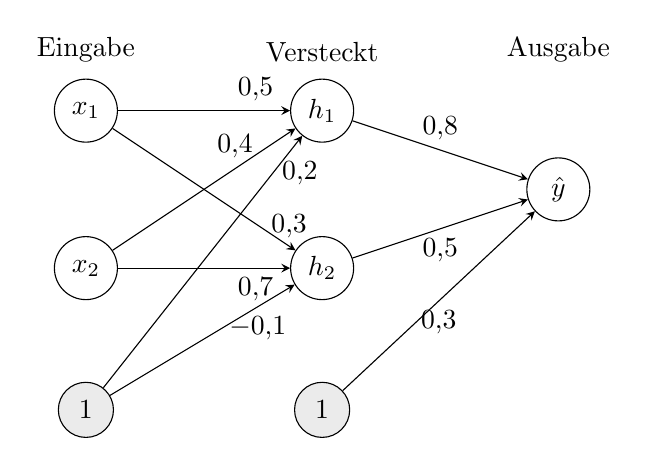
\begin{tikzpicture}[scale=1,
    neuron/.style={circle, draw, minimum size=0.8cm},
    bias/.style={circle, draw, fill=black!8, minimum size=0.7cm},
    >=stealth
]
  \node[neuron] (x1) at (0,1.4)  {$x_1$};
  \node[neuron] (x2) at (0,-0.6) {$x_2$};
  \node[bias]   (b1) at (0,-2.4) {$1$};
  \node[neuron] (h1) at (3,1.4)  {$h_1$};
  \node[neuron] (h2) at (3,-0.6) {$h_2$};
  \node[bias]   (b2) at (3,-2.4) {$1$};
  \node[neuron] (y)  at (6,0.4)  {$\hat{y}$};
  \draw[->] (x1) -- node[pos=0.8, above] {$0{,}5$} (h1);
  \draw[->] (x1) -- node[pos=0.8, right=1pt] {$0{,}3$} (h2);
  \draw[->] (x2) -- node[pos=0.85, left=2pt] {$0{,}4$} (h1);
  \draw[->] (x2) -- node[pos=0.8, below] {$0{,}7$} (h2);
  \draw[->] (b1) -- node[pos=0.85, right] {$0{,}2$} (h1);
  \draw[->] (b1) -- node[pos=0.8, below] {$-0{,}1$} (h2);
  \draw[->] (h1) -- node[above] {$0{,}8$} (y);
  \draw[->] (h2) -- node[below] {$0{,}5$} (y);
  \draw[->] (b2) -- node[below] {$0{,}3$} (y);
  \node[draw=none, above] at (0,1.9) {Eingabe};
  \node[draw=none, above] at (3,1.9) {Versteckt};
  \node[draw=none, above] at (6,1.9) {Ausgabe};
\end{tikzpicture}
\end{center}

Gegeben sei der Input $\mathbf{x} = (1,2)^{\mathsf{T}}$ mit Sollwert $y = 2$
und Lernrate $\alpha = 0{,}1$. Das Bias-Gewicht eines Neurons wird
behandelt wie ein gewöhnliches Gewicht mit konstanter Eingabe $o = 1$.

\begin{enumerate}[label=\alph*)]
  \item Führen Sie die Vorwärtsrechnung durch und bestimmen Sie
        $h_1$, $h_2$ und $\hat{y}$.
  \item Berechnen Sie die Fehlersignale $\delta_j$ nach
        \[
          \delta_j =
          \begin{cases}
            \varphi'(\mathrm{net}_j)\,(\hat{y} - y),
              & j \text{ Ausgabeneuron},\\[0.2cm]
            \varphi'(\mathrm{net}_j)\displaystyle\sum_k \delta_k\,w_{jk},
              & \text{sonst}.
          \end{cases}
        \]
  \item Berechnen Sie die neuen Gewichte \textbf{einschließlich der
        Bias-Gewichte} nach einer Iteration des Gradientenabstiegs
        \[
          w_{ij}' = w_{ij} + \Delta w_{ij},
          \qquad
          \Delta w_{ij} = -\alpha\,\delta_j\,o_i .
        \]
\end{enumerate}
}

\loesung{
\begin{enumerate}[label=\alph*)]
  \item \textbf{Vorwärtsrechnung.} Das Bias-Neuron liefert den konstanten
  Summanden $1\cdot b_j$. Da beide Netzeingaben positiv sind, gilt
  $\varphi(\mathrm{net}) = \mathrm{net}$ für die ReLU-Neuronen:
  \begin{align*}
    h_1 &= \varphi(1\cdot 0{,}5 + 2\cdot 0{,}4 + 1\cdot 0{,}2)
         = \varphi(1{,}5) = 1{,}5,\\
    h_2 &= \varphi(1\cdot 0{,}3 + 2\cdot 0{,}7 + 1\cdot(-0{,}1))
         = \varphi(1{,}6) = 1{,}6,\\
    \hat{y} &= 0{,}8\cdot 1{,}5 + 0{,}5\cdot 1{,}6 + 1\cdot 0{,}3 = 2{,}3 .
  \end{align*}

  \item \textbf{Fehlersignale.} Wegen $\varphi'(\mathrm{net}_j) = 1$ für
  die Identität und für ReLU bei positiver Netzeingabe:
  \begin{align*}
    \delta_{\hat{y}} &= 1\cdot(2{,}3 - 2) = 0{,}3,\\
    \delta_{h_1} &= 1\cdot \delta_{\hat{y}}\,w_{h_1\hat{y}}
                  = 0{,}3\cdot 0{,}8 = 0{,}24,\\
    \delta_{h_2} &= 1\cdot \delta_{\hat{y}}\,w_{h_2\hat{y}}
                  = 0{,}3\cdot 0{,}5 = 0{,}15 .
  \end{align*}
  Die Fehlersignale der Bias-Neuronen müssen nicht berechnet werden, da
  sie keine eingehenden Verbindungen besitzen.

  \item \textbf{Gewichtsaktualisierung.} Für die Bias-Gewichte ist die
  zugehörige Eingabe $o = 1$.

  \textbf{Versteckt $\to$ Ausgabe (inkl. Bias):}
  \begin{align*}
    \Delta w_{h_1\hat{y}} &= -0{,}1\cdot 0{,}3\cdot 1{,}5 = -0{,}045,
      & w_{h_1\hat{y}}' &= 0{,}8 - 0{,}045 = 0{,}755,\\
    \Delta w_{h_2\hat{y}} &= -0{,}1\cdot 0{,}3\cdot 1{,}6 = -0{,}048,
      & w_{h_2\hat{y}}' &= 0{,}5 - 0{,}048 = 0{,}452,\\
    \Delta b_{\hat{y}} &= -0{,}1\cdot 0{,}3\cdot 1 = -0{,}03,
      & b_{\hat{y}}' &= 0{,}3 - 0{,}03 = 0{,}27 .
  \end{align*}

  \textbf{Eingabe $\to$ Versteckt (inkl. Bias):}
  \begin{align*}
    \Delta w_{x_1 h_1} &= -0{,}1\cdot 0{,}24\cdot 1 = -0{,}024,
      & w_{x_1 h_1}' &= 0{,}5 - 0{,}024 = 0{,}476,\\
    \Delta w_{x_2 h_1} &= -0{,}1\cdot 0{,}24\cdot 2 = -0{,}048,
      & w_{x_2 h_1}' &= 0{,}4 - 0{,}048 = 0{,}352,\\
    \Delta b_{h_1} &= -0{,}1\cdot 0{,}24\cdot 1 = -0{,}024,
      & b_{h_1}' &= 0{,}2 - 0{,}024 = 0{,}176,\\
    \Delta w_{x_1 h_2} &= -0{,}1\cdot 0{,}15\cdot 1 = -0{,}015,
      & w_{x_1 h_2}' &= 0{,}3 - 0{,}015 = 0{,}285,\\
    \Delta w_{x_2 h_2} &= -0{,}1\cdot 0{,}15\cdot 2 = -0{,}03,
      & w_{x_2 h_2}' &= 0{,}7 - 0{,}03 = 0{,}67,\\
    \Delta b_{h_2} &= -0{,}1\cdot 0{,}15\cdot 1 = -0{,}015,
      & b_{h_2}' &= -0{,}1 - 0{,}015 = -0{,}115 .
  \end{align*}

  Da $\hat{y} = 2{,}3 > 2 = y$ war, ist der Fehler positiv und sämtliche
  Gewichte samt Bias werden verkleinert, sodass $\hat{y}$ sinkt.
\end{enumerate}
}



% -------------------------------------------------------------------
% 14) Netzgroesse, Batches und Epochen
% -------------------------------------------------------------------
\aufgabe{
Ein MLP besitzt $4$ Eingangsneuronen, zwei Hidden-Layer mit $6$ bzw. $5$
Neuronen und $3$ Ausgabeneuronen. Jede Schicht außer der Ausgabeschicht
besitzt zusätzlich ein Bias-Neuron.

\begin{enumerate}[label=\alph*)]
  \item Geben Sie die Dimensionen von $W^{(1)}$, $W^{(2)}$ und $W^{(3)}$ an
        und berechnen Sie die Gesamtzahl der Gewichte.
  \item Das Netz wird mit $50\,000$ Beispielen bei einer Batch-Größe von
        $200$ über $30$ Epochen trainiert. Wie viele Iterationsschritte
        (Gewichts-Updates) ergeben sich?
\end{enumerate}
}

\loesung{
\begin{enumerate}[label=\alph*)]
  \item Jede Matrix bildet die um das Bias-Neuron erweiterte Vorgängerschicht
  auf die Folgeschicht ab:
  \[
    W^{(1)} \in \mathbb{R}^{6\times 5}, \qquad
    W^{(2)} \in \mathbb{R}^{5\times 7}, \qquad
    W^{(3)} \in \mathbb{R}^{3\times 6}
  \]
  \[
    6\cdot 5 + 5\cdot 7 + 3\cdot 6 = 30 + 35 + 18 = \textbf{83}
  \]

  \item Iterationen pro Epoche:
  \[
    \frac{50\,000}{200} = 250
  \]
  Insgesamt:
  \[
    250\cdot 30 = \textbf{7500} \text{ Gewichts-Updates}
  \]
\end{enumerate}
}